\documentclass[fleqn,10pt]{wlscirep}
\usepackage[utf8]{inputenc}
\usepackage[T1]{fontenc}
\usepackage{lineno}
\linenumbers

\title{Microephys: Extending the Brain Imaging Data Structure specification to animal microelectrode electrophysiology}

\author[1,$\dag$]{Alice Author}
\author[2,$\dag$]{Bob Author}
\author[1,2]{Christine Author}
\author[2,*]{Derek Author}
\affil[1]{Affiliation, department, city, postcode, country}
\affil[2]{Affiliation, department, city, postcode, country}

\affil[*]{corresponding author(s): Derek Author (corresponding.author@email.example)}

\affil[$\dag$]{these authors contributed equally to this work}


\begin{abstract}
% This is a manuscript template for Data Descriptor submissions to \emph{Scientific Data} (\href{http://www.nature.com/scientificdata}{http://www.nature.com/scientificdata}). The abstract must be no longer than 170 words, and should succinctly describe the study, the assay(s) performed, the resulting data, and the reuse potential, but should not make any claims regarding new scientific findings. No references are allowed in this section. 

% Taken from Christian's submission to INCF Assembly 2024 for intiating discussions
Standards-compliance is a crucial aspect of open science, as it facilitates both collaboration and transparency.
The Brain Imaging Data Structure (BIDS) is an increasingly widely used set of specifications, and is being actively expanded beyond its initial scope of brain imaging.
Animal research methods have received increasing attention in BIDS, and among these, electrophysiological methods have been of considerable interest.
Here we present the extension of BIDS to “microelectrode electrophysiology”, a term coined to denote electrophysiological recordings with microelectrodes, including intracellular, extracellular, and tissue-level electrophysiology.
This BIDS extension proposal, BEP 032, deals with the challenges arising from the diverse range of technologies in electrophysiology and converges on signal and electrode channels as common metadata denominators, with the open standards NIX and NWB as allowed data formats.
It provides a homogeneous standard for various microelectrode techniques, including patch clamp and multielectrode  array recordings.
Moreover, it tackles integration with behavioural data and electrode localization specifications.
The directory layout is consistent with BIDS, allowing intuitive data structure recognition at-a-glance even for non-experts.
Our work provides not only access to cutting-edge standards for researchers in electrophysiology, but also a crucial extension to BIDS, providing a handling template for metadata aspects with relevance beyond electrophysiology.

\end{abstract}
\begin{document}

\flushbottom
\maketitle
%  Click the title above to edit the author information and abstract

\thispagestyle{empty}

% \noindent Please note: Abbreviations should be introduced at the first mention in the main text – no abbreviations lists or tables should be included. Structure of the main text is provided below.

\section*{Background \& Summary}

% (700 words maximum) An overview of the study design, the assay(s) performed, and the created data, including any background information needed to put this study in the context of previous work and the literature. The section should also briefly outline the broader goals that motivated the creation of this dataset and the potential reuse value. We also encourage authors to include a figure that provides a schematic overview of the study and assay(s) design. The Background \& Summary should not include subheadings. This section and the other main body sections of the manuscript should include citations to the literature as needed. 

There have been significant developments in neuroimaging and electrophysiology techniques used in neuroscience over the last few years. Imaging techniques such as MRI, fMRI, or PET provide detailed brain activity maps across space. On the other hand, understanding neuronal dynamics requires high-resolution electrophysiological methods, including extracellular and intracellular recording.

Efforts are being made to standardize these heterogeneous datasets generated by micro-electrode electrophysiology techniques, making both a need for this and the benefits more visible. These methods involve using language-agnostic common object data models (see Neo), and comprehensive data formats (see NWB, NIX, ABF, NDF, OpenEphys etc.) [add more]. While these strategies call attention to the significance of standardization, they also suggest that there is fragmentation within current efforts, which needs to be addressed through a unified and intuitive approach that encourages widespread adoption.

In this context, we propose an extension of the Brain Imaging Data Structure (BIDS) – a standard that has already gained wide acceptance – to incorporate “microelectrode electrophysiology, " including intracellular, extracellular, and tissue-level electrophysiology.

\section*{Methods}

% The Methods should include detailed text describing any steps or procedures used in producing the data, including full descriptions of the experimental design, data acquisition assays, and any computational processing (e.g. normalization, image feature extraction). See the detailed section in our submission guidelines for advice on writing a transparent and reproducible methods section. Related methods should be grouped under corresponding subheadings where possible, and methods should be described in enough detail to allow other researchers to interpret and repeat, if required, the full study. Specific data outputs should be explicitly referenced via data citation (see Data Records and Citing Data, below).

% Authors should cite previous descriptions of the methods under use, but ideally the method descriptions should be complete enough for others to understand and reproduce the methods and processing steps without referring to associated publications. There is no limit to the length of the Methods section. Subheadings should not be numbered.

% \subsection*{Subsection}

% Example text under a subsection. Bulleted lists may be used where appropriate, e.g.

% \begin{itemize}
% \item First item
% \item Second item
% \end{itemize}

% \subsubsection*{Third-level section}

\subsection*{Modality and Data Type Nomenclature}
% This section tries to summarize discussions on the topic and justify the nomenclature we decided on
% TODO: Do we add more arguments for some of the rejected options like 'Cellular'?
% Refer discussions from here: https://github.com/bids-standard/bids-specification/issues/1800
% Ontologies and terminologies: https://openminds-documentation.readthedocs.io/en/latest/instance_libraries/terminologies/technique.html#extracellularelectrophysiology
% https://ontobee.org/ontology/OBI?iri=http://purl.obolibrary.org/obo/OBI_0000454
% https://scicrunch.org/scicrunch/interlex/view/ilx_0739521
The modality described in this extension and that characterizes the introduced datasets is termed 'Microelectrode Electrophysiology'. This choice balances specificity, clarity and alignment with the current BIDS standard and common community usage.

\subsubsection*{BIDS Terminology}
% These definitions are copied over for now from BIDS spec
\begin{itemize}
    \item Modality: The category of brain data recorded by a file. For MRI data, different pulse sequences are considered distinct modalities, such as T1w, bold or dwi. For passive recording techniques, such as EEG, MEG or iEEG, the technique is sufficiently uniform to define the modalities eeg, meg and ieeg. When applicable, the modality is indicated in the suffix. The modality may overlap with, but should not be confused with the data type.
    \item Data type: A functional group of different types of data. Data files are contained in a directory named for the data type. In raw datasets, the data type directory is nested inside subject and (optionally) session directories.
    \item Suffix: An alphanumeric string that is part of a filename, located after all entities and following a final \texttt{\_}, right before the file extension. For example, it is \texttt{eeg} in \texttt{sub-05\_task-matchingpennies\_eeg.vhdr}.
\end{itemize}

\subsubsection*{Specificity and Distinction from Existing Modalities}
Microelectrode electrophysiology establishes a clear distinction from other electrophysiological recording techniques already described by BIDS, such as EEG and iEEG, with the term 'micro' referring to the typical spatial scale of electrode contacts. Hence, the modality name differentiates these recordings from broader electrophysiological categories while maintaining clarity and agreement with the conventional community usage.

% https://github.com/bids-standard/bids-specification/issues/1800
% https://docs.google.com/document/d/1GlHr3Go5sR2o_zmxyCU6Sq1W1LLAaV_XZcKpeG_iBFw/edit?tab=t.0

\subsubsection*{Maintaining Modularity and Extensibility of BIDS}
The proposed choice is a foresighted approach for maintaining the modularity and extensibility of BIDS. As new electrophysiological techniques are introduced in the future, a specific and descriptive naming convention would help prevent probable namespace conflicts, ensuring new modalities and data types can integrate seamlessly without breaking the current standard.


\subsubsection*{Separation of Data types and Suffixes}
As for the datatype, we introduce "icephys" for intracellular electrophysiology and "ecephys" for extracellular electrophysiology. BIDS datatypes categorize functional groups of data and metadata files and subsequently serve as the directory name.

\subsection*{Related BIDS Modalities}


\subsection*{Data Types: icephys and ecephys}
\section*{Participant keyfile}
\subsection*{Surgery Information}
Note from 20250820 Meeting: Review compatibility with AIND (https://aind-data-schema.readthedocs.io/en/stable/acquisition.html) schema
\subsection*{Age and Birthdate}
\section*{Probes, Electrodes, and Channels}
\subsection*{Electrode Locations}
\subsubsection*{Coordinate system}
\subsubsection*{Electrode Placement Image}
\subsection*{Channel type enum additions}
\section*{Multipart recordings}
\subsection*{scans.tsv}
\subsection*{events.tsv}
\section*{Data Formats for recorded data}
\subsection*{NWB}
\subsection*{NIX}
\section*{Example Datasets}
\section*{Community Software and Adoption}
 
% Topical subheadings are allowed.

\section*{Data Records}

% The Data Records section should be used to explain each data record associated with this work, including the repository where this information is stored, and to provide an overview of the data files and their formats. Each external data record should be cited numerically in the text of this section, for example \cite{Hao:gidmaps:2014}, and included in the main reference list as described below. A data citation should also be placed in the subsection of the Methods containing the data-collection or analytical procedure(s) used to derive the corresponding record. Providing a direct link to the dataset may also be helpful to readers (\hyperlink{https://doi.org/10.6084/m9.figshare.853801}{https://doi.org/10.6084/m9.figshare.853801}).

% Tables should be used to support the data records, and should clearly indicate the samples and subjects (study inputs), their provenance, and the experimental manipulations performed on each (please see 'Tables' below). They should also specify the data output resulting from each data-collection or analytical step, should these form part of the archived record.

\section*{Technical Validation}

% This section presents any experiments or analyses that are needed to support the technical quality of the dataset. This section may be supported by figures and tables, as needed. This is a required section; authors must present information justifying the reliability of their data.

\section*{Usage Notes}

% The Usage Notes should contain brief instructions to assist other researchers with reuse of the data. This may include discussion of software packages that are suitable for analysing the assay data files, suggested downstream processing steps (e.g. normalization, etc.), or tips for integrating or comparing the data records with other datasets. Authors are encouraged to provide code, programs or data-processing workflows if they may help others understand or use the data. Please see our code availability policy for advice on supplying custom code alongside Data Descriptor manuscripts.

% For studies involving privacy or safety controls on public access to the data, this section should describe in detail these controls, including how authors can apply to access the data, what criteria will be used to determine who may access the data, and any limitations on data use. 

\section*{Code availability}

% For all studies using custom code in the generation or processing of datasets, a statement must be included under the heading "Code availability", indicating whether and how the code can be accessed, including any restrictions to access. This section should also include information on the versions of any software used, if relevant, and any specific variables or parameters used to generate, test, or process the current dataset. 

\bibliography{sample}

% \noindent LaTeX formats citations and references automatically using the bibliography records in your .bib file, which you can edit via the project menu. Use the cite command for an inline citation, e.g. \cite{Kaufman2020, Figueredo:2009dg, Babichev2002, behringer2014manipulating}. For data citations of datasets uploaded to e.g. \emph{figshare}, please use the \verb|howpublished| option in the bib entry to specify the platform and the link, as in the \verb|Hao:gidmaps:2014| example in the sample bibliography file. For journal articles, DOIs should be included for works in press that do not yet have volume or page numbers. For other journal articles, DOIs should be included uniformly for all articles or not at all. We recommend that you encode all DOIs in your bibtex database as full URLs, e.g. https://doi.org/10.1007/s12110-009-9068-2.

\section*{Acknowledgements} (not compulsory)

% Acknowledgements should be brief, and should not include thanks to anonymous referees and editors, or effusive comments. Grant or contribution numbers may be acknowledged.

\section*{Author contributions statement}

% Must include all authors, identified by initials, for example:
% A.A. conceived the experiment(s), A.A. and B.A. conducted the experiment(s), C.A. and D.A. analysed the results. All authors reviewed the manuscript. 

\section*{Competing interests} (mandatory statement)

% The corresponding author is responsible for providing a \href{https://www.nature.com/sdata/policies/editorial-and-publishing-policies#competing}{competing interests statement} on behalf of all authors of the paper. This statement must be included in the submitted article file.

\section*{Figures \& Tables}

% Figures, tables, and their legends, should be included at the end of the document. Figures and tables can be referenced in \LaTeX{} using the ref command, e.g. Figure \ref{fig:stream} and Table \ref{tab:example}. 

% Authors are encouraged to provide one or more tables that provide basic information on the main ‘inputs’ to the study (e.g. samples, participants, or information sources) and the main data outputs of the study. Tables in the manuscript should generally not be used to present primary data (i.e. measurements). Tables containing primary data should be submitted to an appropriate data repository.

% Tables may be provided within the \LaTeX{} document or as separate files (tab-delimited text or Excel files). Legends, where needed, should be included here. Generally, a Data Descriptor should have fewer than ten Tables, but more may be allowed when needed. Tables may be of any size, but only Tables which fit onto a single printed page will be included in the PDF version of the article (up to a maximum of three). 

% Due to typesetting constraints, tables that do not fit onto a single A4 page cannot be included in the PDF version of the article and will be made available in the online version only. Any such tables must be labelled in the text as ‘Online-only’ tables and numbered separately from the main table list e.g. ‘Table 1, Table 2, Online-only Table 1’ etc.

% \begin{figure}[ht]
% \centering
% 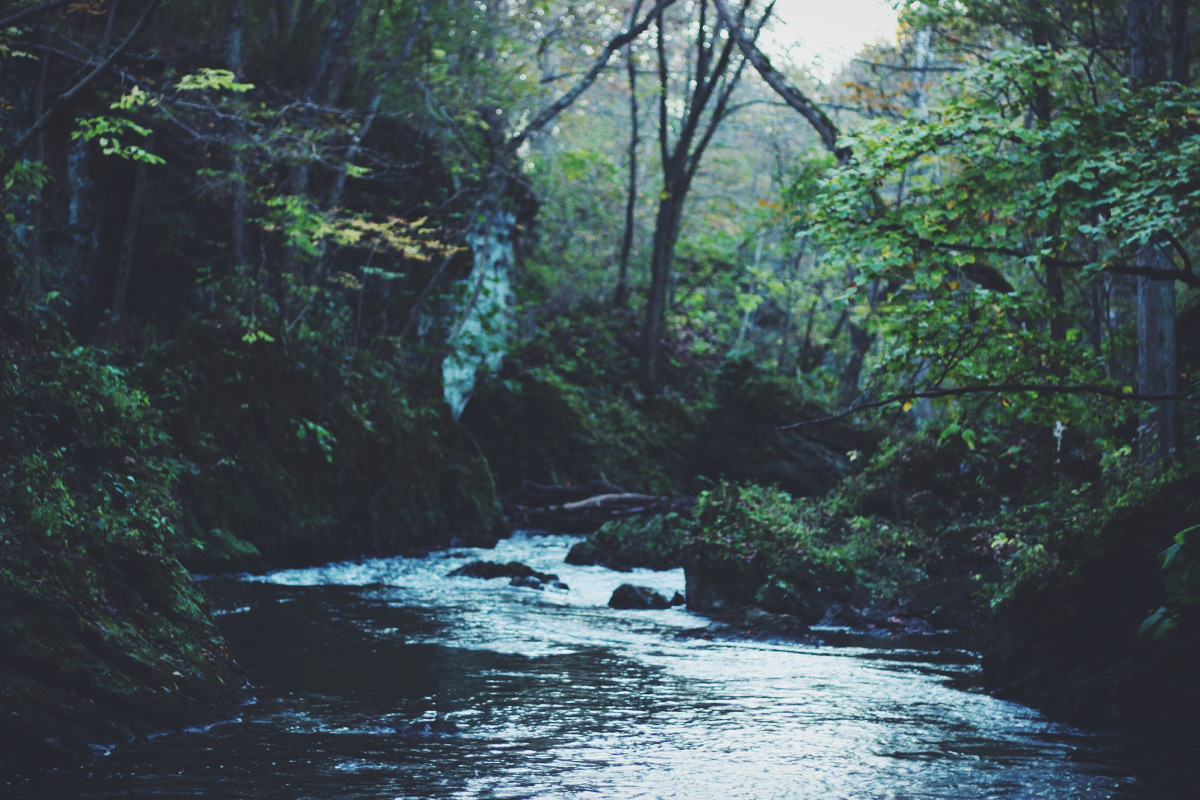
\includegraphics[width=\linewidth]{stream}
% \caption{Legend (350 words max). Example legend text.}
% \label{fig:stream}
% \end{figure}

% \begin{table}[ht]
% \centering
% \begin{tabular}{|l|l|l|}
% \hline
% Condition & n & p \\
% \hline
% A & 5 & 0.1 \\
% \hline
% B & 10 & 0.01 \\
% \hline
% \end{tabular}
% \caption{\label{tab:example}Legend (350 words max). Example legend text.}
% \end{table}

\end{document}